\documentclass{article}
\title{CUDA Parallel Programming\\Homework 6}
\usepackage{graphicx}
\usepackage[UTF8]{ctex}
\usepackage{hyperref}
\usepackage{amsmath}
\CTEXoptions[today=old]
\author{40647007S 朱健愷}

\begin{document}
	\maketitle
	\section{Source codes}
	\subsection{File Layout}
	\begin{itemize}
		\item monteCarlo\textunderscore{NGPU}/monteCarlo\textunderscore{ss}\textunderscore{ngpu}.cu - Main code computes the integral using simple sampling monte carlo simulation in both CPU and GPU.
		\item 		\item monteCarlo\textunderscore{NGPU}/monteCarlo\textunderscore{mis}\textunderscore{ngpu}.cu - Main code computes the integral using importance sampling with metropolis algorithm monte carlo simulation in both CPU and GPU.
		\item Makefile - Script to auto generate executable from code.
		\item monteCarlo\textunderscore{NGPU}/experiment.sh - Script to auto generate results of the integral using both CPU and GPU, simple sampling and importance sampling with metropolis algorithm monte carlo simulation. Its statistical result using different block size are also taken into experiment's consideration.
		\item monteCarlo\textunderscore{NGPU}/result/ss/GPU\textunderscore*/N\textunderscore{*}\textunderscore{block}\textunderscore*/Output - Output CPU and GPU compute result of the integral using simple sampling monte carlo simulation, the number behind GPU is the number of GPU it used to generate the result, the number behind N is the $2^N$ samples it generated and used in integral, the number behind block is the block size I assigned to perform the experiment.
		\item monteCarlo\textunderscore{NGPU}/result/mis/GPU\textunderscore*/N\textunderscore{*}\textunderscore{block}\textunderscore*/Output - Output CPU and GPU compute result of the integral using importance sampling with metropolis algorithm monte carlo simulation, the number behind GPU is the number of GPU it used to generate the result, the number behind N is the $2^N$ samples it generated and used in integral, the number behind block is the block size I assigned to perform the experiment.		
		\item notebook/*.png - Plots concluding output result
	\end{itemize}
	
	
	\subsection{Usage}
	Make code in both monteCarlo\textunderscore{NGPU}/ directory
	Run the experiment.sh script in monteCarlo\textunderscore{NGPU}/ directory
	
	\begin{verbatim}
	cd monteCarlo_NGPU
	make
	sh experiment.sh
	\end{verbatim}
	
	And it will produce the integral using both simple sampling and importance sampling with metropolis algorithm statistical result using different block size.
	
	\section{Code design}
	\subsection{Simple sampling Monte Carlo Simulation}
	For simple sampling monta carlo simulation, I used uniform sampling on sample point $x_i$ which each dimension of it distribute in range $[0, 1]$ uniformly, and calculate the mean of the function value with sample point using 
	\begin{equation}
		\frac{\Sigma_i{f(x_i)}}{N}
	\end{equation}
	where $i$ denotes $i^{th}$ sample point, N denotes total sample point amount.
	Calculating standard deviation of the function value with sample point using 
	\begin{equation}
		\sqrt{\frac{\frac{1}{N}\Sigma_i{f(x_i)^2}-(\frac{1}{N}\Sigma_i{f(x_i)})^2}{N}}
	\end{equation}
	where $i$ denotes $i^{th}$ sample point, N denotes total sample point amount.
	
	I implemented both CPU code and GPU code to perform the simple sampling, the GPU code is simply collecting the mean and standard deviation from CPU generated sample points.

	\subsection{Importance sampling with Metropolis algorithm Monte Carlo Simulation}
	For importance sampling with metropolis algorithm monta carlo simulation, I used importance sampling on sample point $x_i$ which each dimension of it distribute in range $[0, 1]$ according to weighting function 
	\begin{equation}
		W(x_1, x_2..., x_10)=w(x_1)w(x_2)...w(x_10), w(x_i)=Ce^{-ax_i}, i=1, ..., 10
	\end{equation}
	Because I want to normalize the weighting function to simplify the following calculation, so I manually choose the $a$ to be 0.001, and $C$ to be
	$\frac{-a}{e^{-a}-1}$, it is derived from
	\begin{equation}
		\int_{0}^{1}w(x)dx=1
	\end{equation}
	After integration, it became
	\begin{equation}
		\frac{Ce^{-a}-C}{-a}=1
	\end{equation}
	Rearranging them gives
	\begin{equation}
		C=\frac{-a}{e^{-a}-1}
	\end{equation}

	To transform the function to be smooth, I calculate the sample point generation function derived from weighting function
	\begin{equation}
		y=\int_0^x w(t)dt=\frac{Ce^{-ax}-C}{-a}
	\end{equation}
	\begin{equation}
		\label{eq:wf}
		x=\frac{\ln(\frac{-a}{C}*y+1)}{-a}
	\end{equation}
	In metropolis algorithm, I first generate the sample points according to weighting function giving uniform distribution as y and get x corresponding to weighting function distribution according to (\ref{eq:wf}) as $X_old$, and calculate its weight $w_old$ using weighting function, and then calculate the next sample point using metropolis algorithm according to teacher's slide. Once obtained the next sample point, I calculate the mean and the standard deviation of the function value with sample point  using 
	\begin{equation}
		\frac{\Sigma_i{\frac{f(x_i)}{w(x_i)}}}{N}
	\end{equation}
	where $i$ denotes $i^{th}$ sample point, N denotes total sample point amount, $w(x)$ denotes the weighting function.
	Calculating standard deviation of the function value with sample point using 
	\begin{equation}
		\sqrt{\frac{\frac{1}{N}\Sigma_i({\frac{f(x_i)}{w(x_i)}^2)}-(\frac{1}{N}\Sigma_i{\frac{f(x_i)}{w(x_i)}})^2}{N}}
	\end{equation}
	where $i$ denotes $i^{th}$ sample point, N denotes total sample point amount, $w(x)$ denotes the weighting function.
	
	I only implemented CPU code to perform the importance sampling with metropolis algorithm, what GPU code remain is intended to provide the timing utility to calculate the time CPU code elapsed.

	\section{Result}
	\subsection{Experiment environment}
	I ran my code on workstation provided in course, below is the Setup of workstation
	\begin{itemize}
		\item Operating system: Linux version 4.19.172 (root@twcp1)\\(gcc version 6.3.0 20170516 (Debian 6.3.0-18+deb9u1))
		\item CPU: Intel(R) Core(TM) i7-4790 CPU @ 3.60GHz
		\item GPU: Nvidia GTX 1060 6GB
		\item Memory: 32GB 
	\end{itemize}
	\subsection{Performance}
	Below two figures showed CPU processing time of both simple sampling monte carlo simulation and importance sampling with metropolis algorithm monte carlo simulation changing sample point amounts.
	\begin{figure}[hb!]
		\centering
		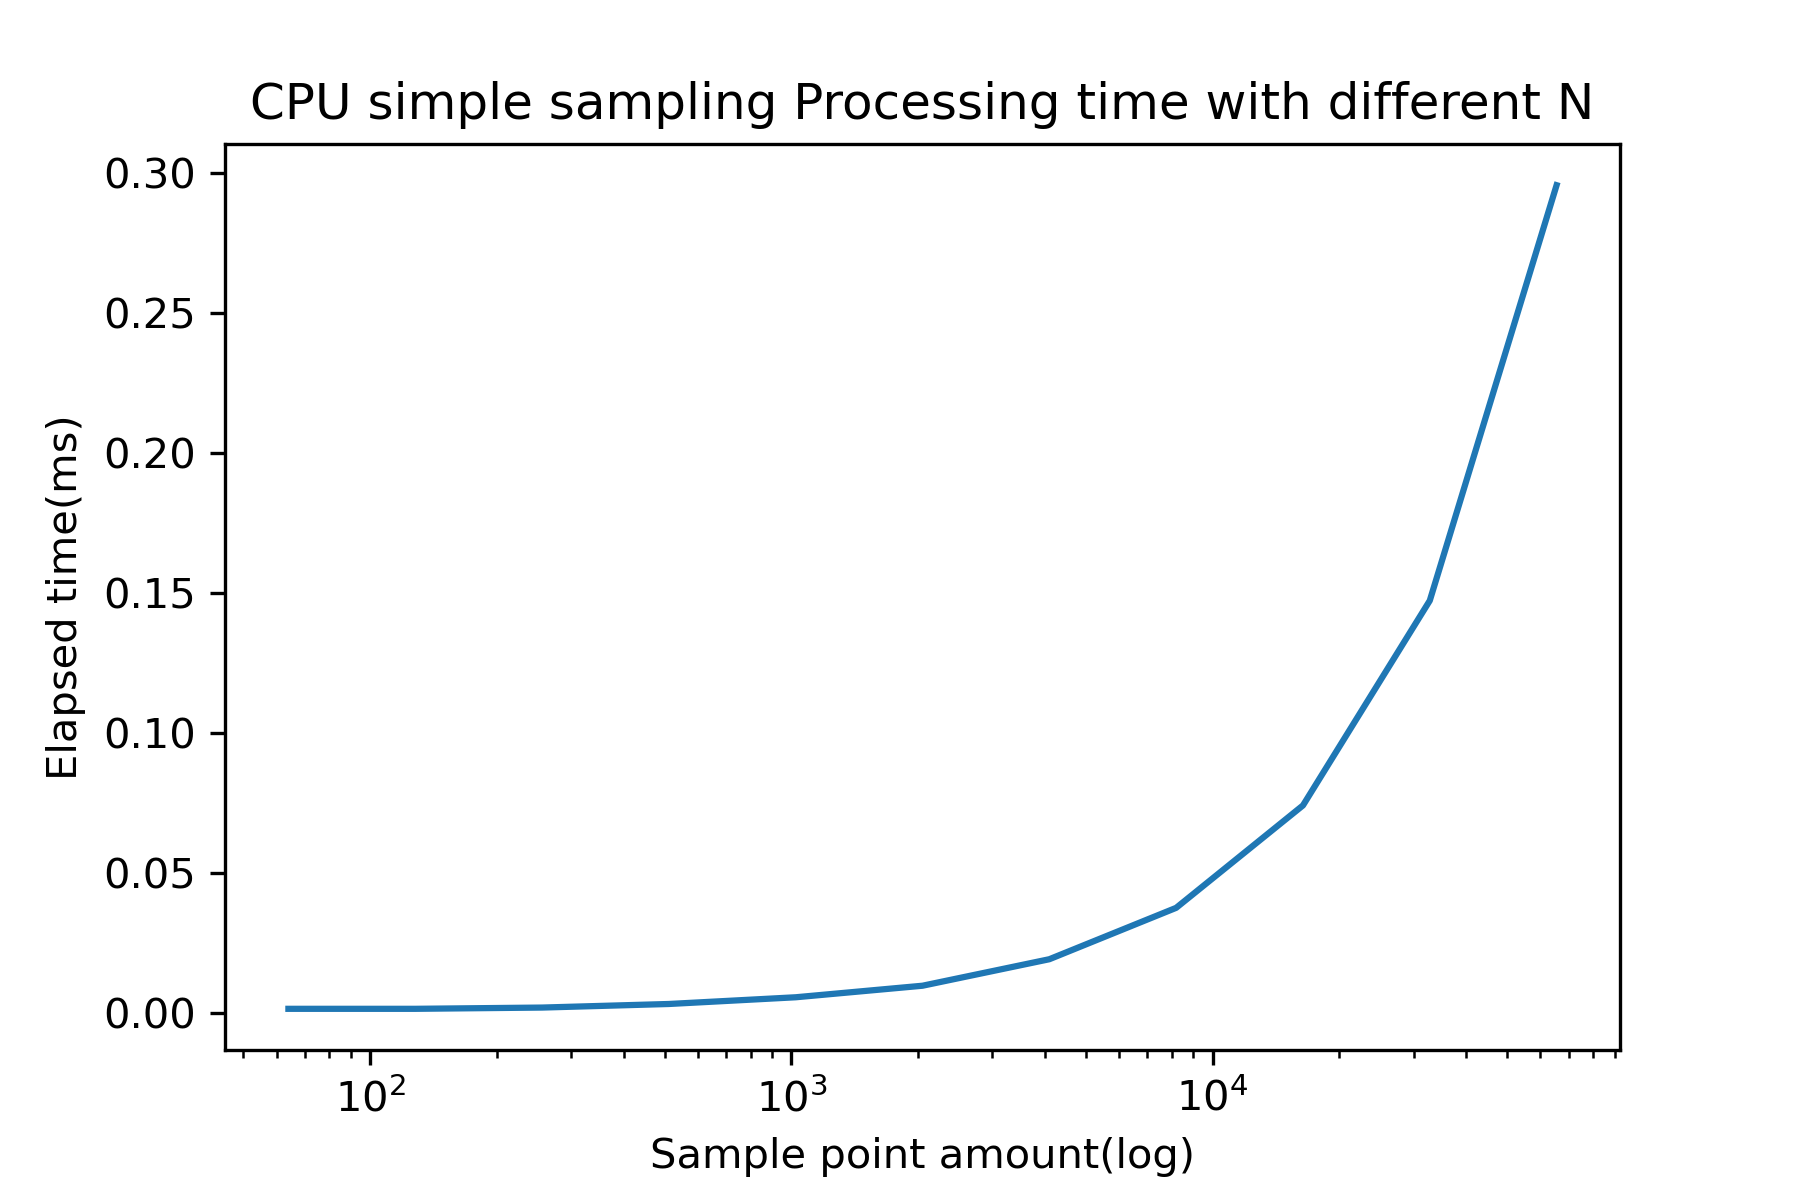
\includegraphics[width=0.9\linewidth]{notebook/cpu_ss}
	\end{figure}
	\begin{figure}[hb!]
		\centering
		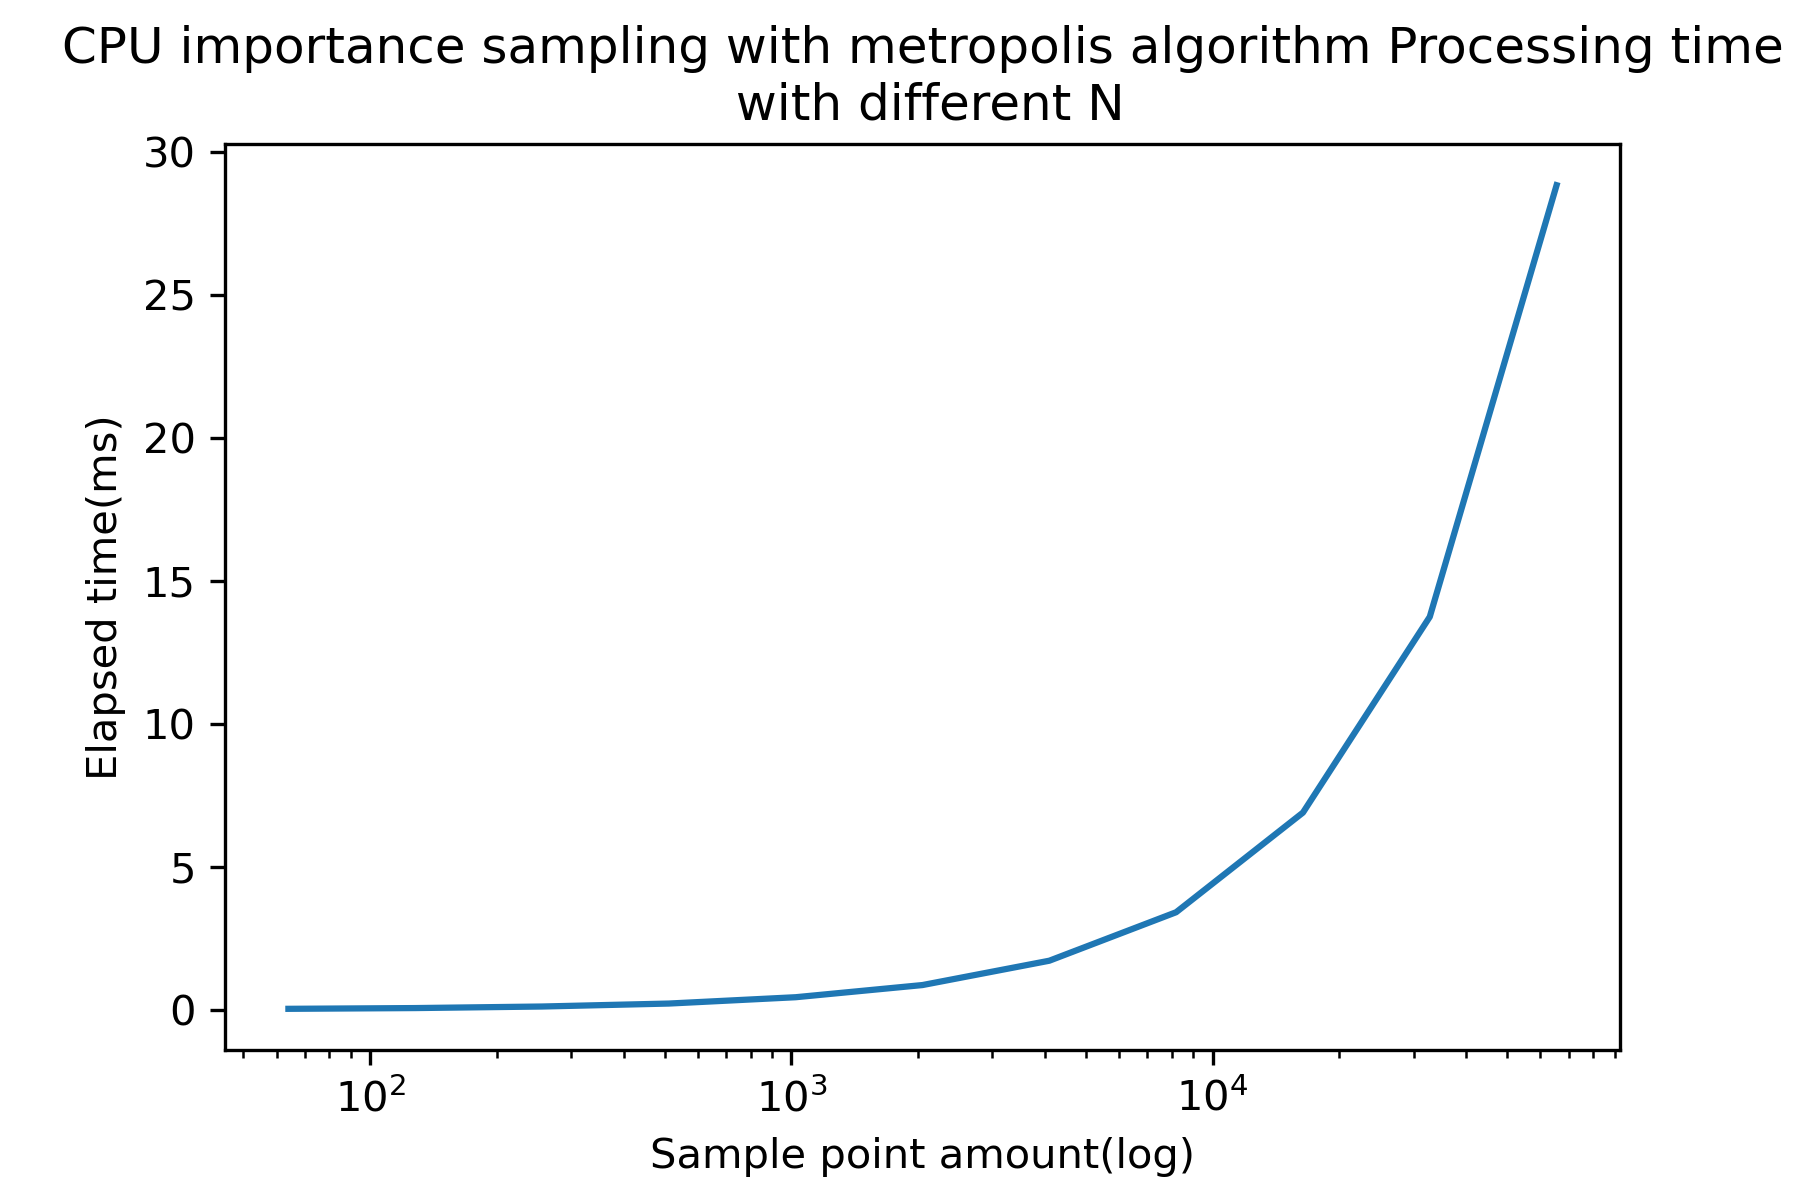
\includegraphics[width=0.9\linewidth]{notebook/cpu_mis}
	\end{figure}
	\newpage
	
	And below two figure showed GPU processing time of simple sampling monte carlo simulation with 1 GPU and 2 GPU changing sample point amounts.
	\begin{figure}[hb!]
		\centering
		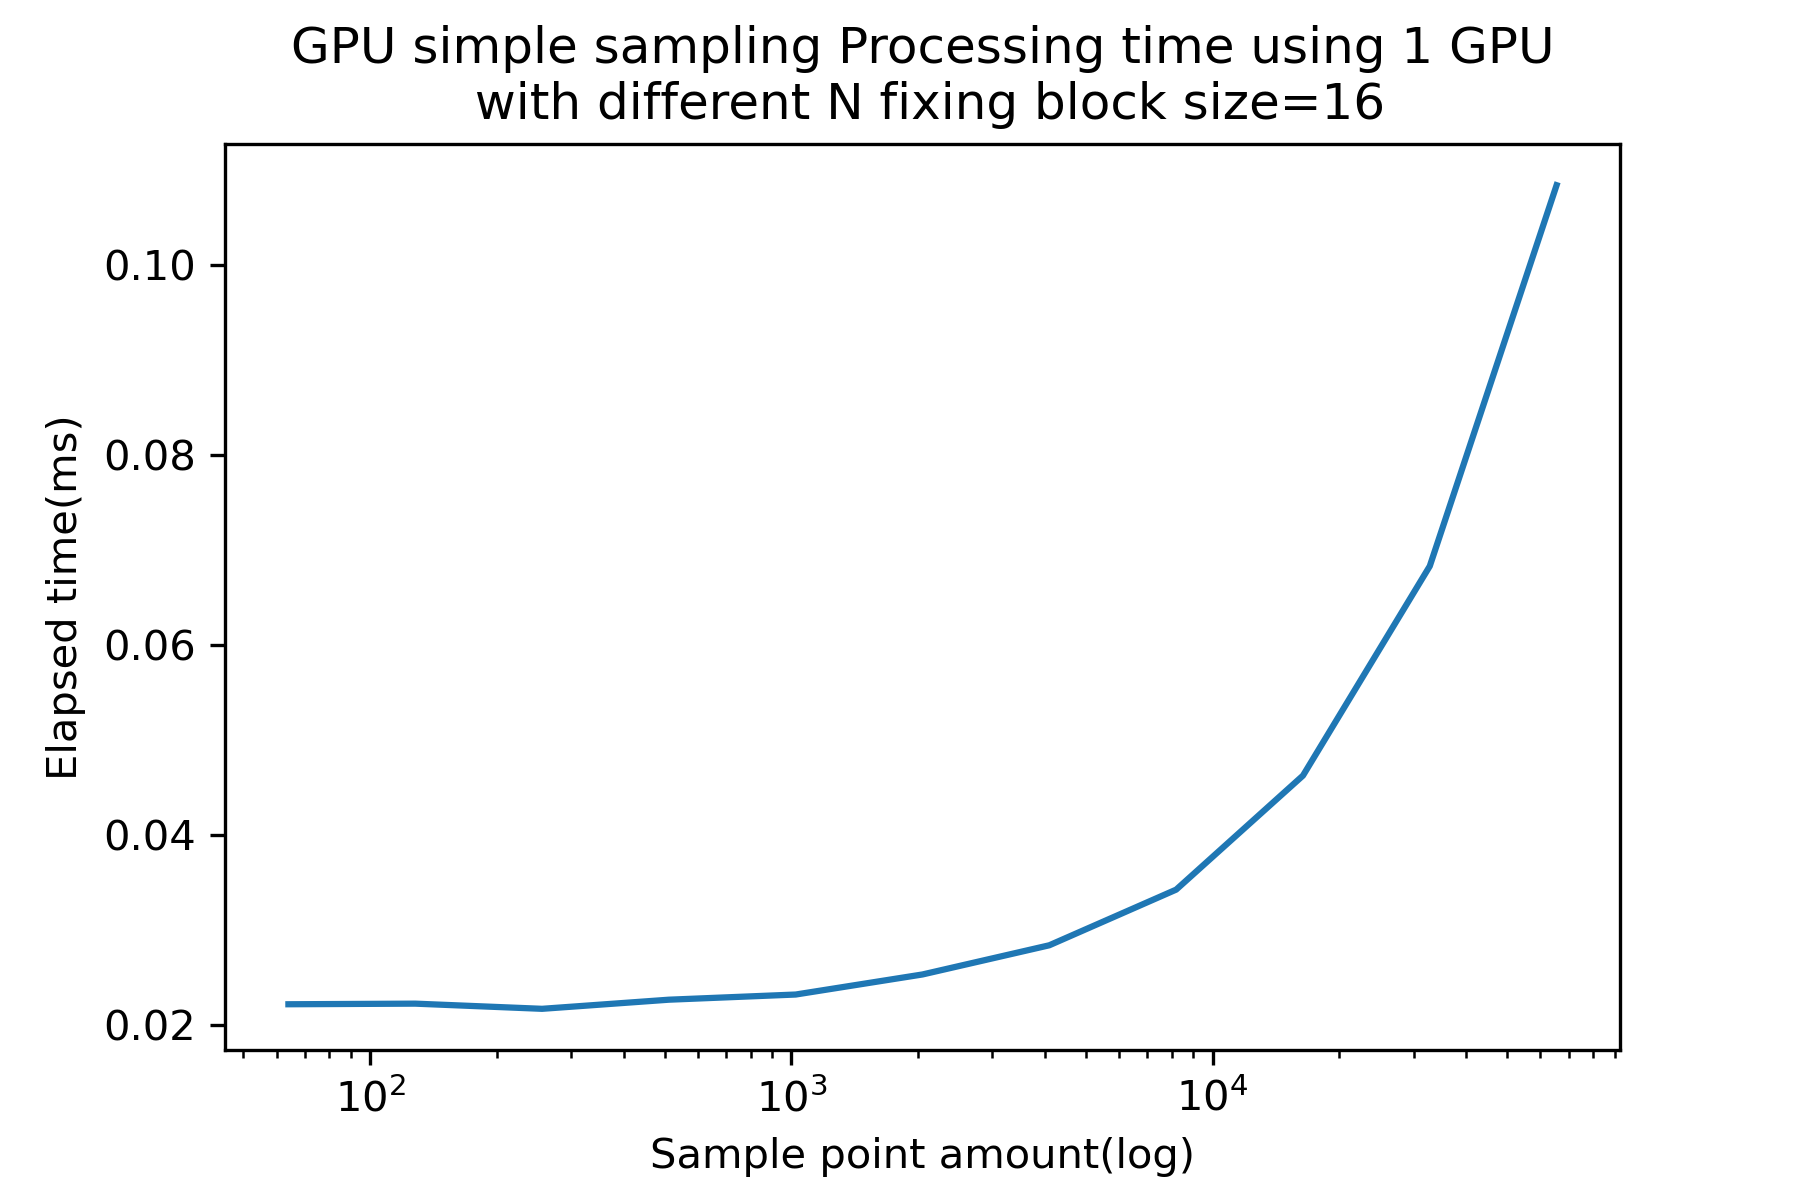
\includegraphics[width=\linewidth]{notebook/1gpu_ss}
	\end{figure}
	\begin{figure}[hb!]
	\centering
	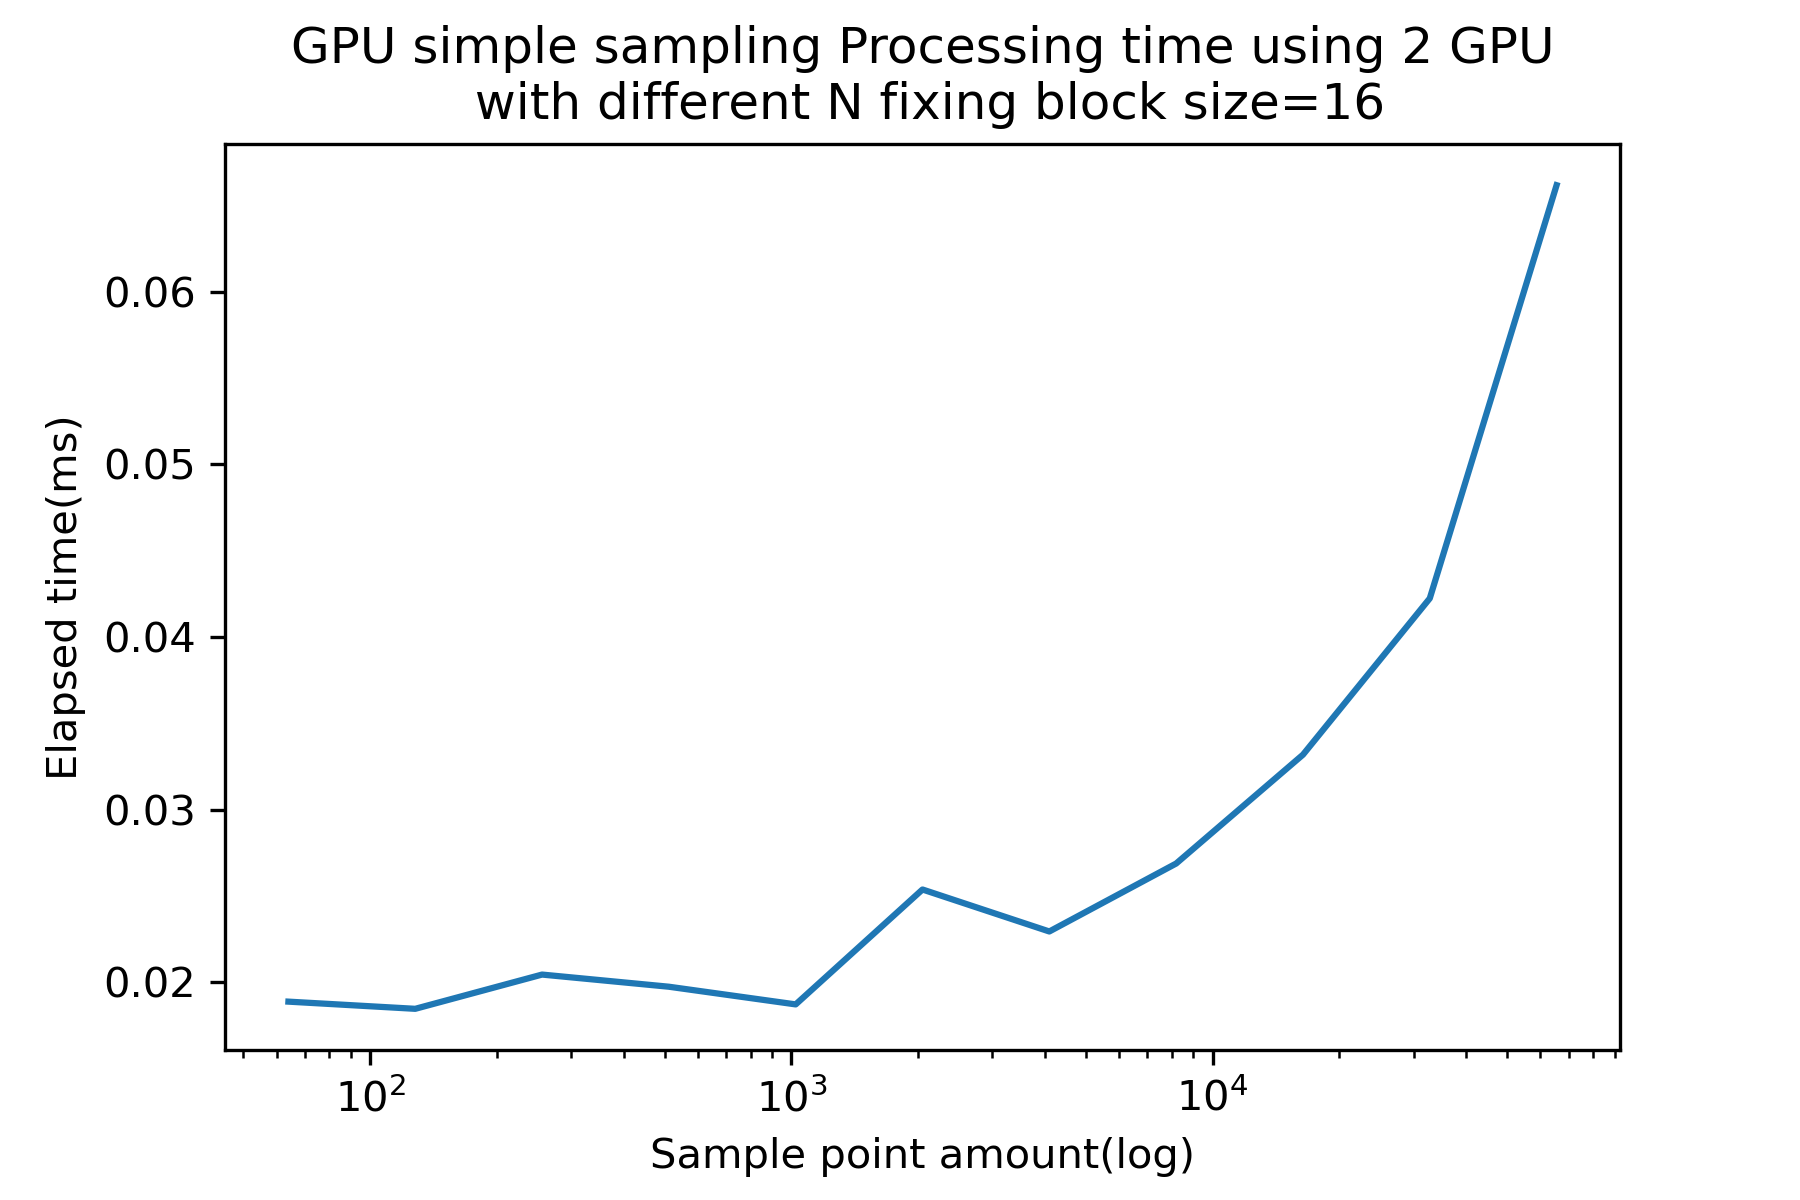
\includegraphics[width=\linewidth]{notebook/2gpu_ss}
	\end{figure}

	The below two figure showed the function value mean of both simple sampling monte carlo simulation and importance sampling with metropolis algorithm monte carlo simulation changing sample point amounts.
	\begin{figure}[hb!]
		\centering
		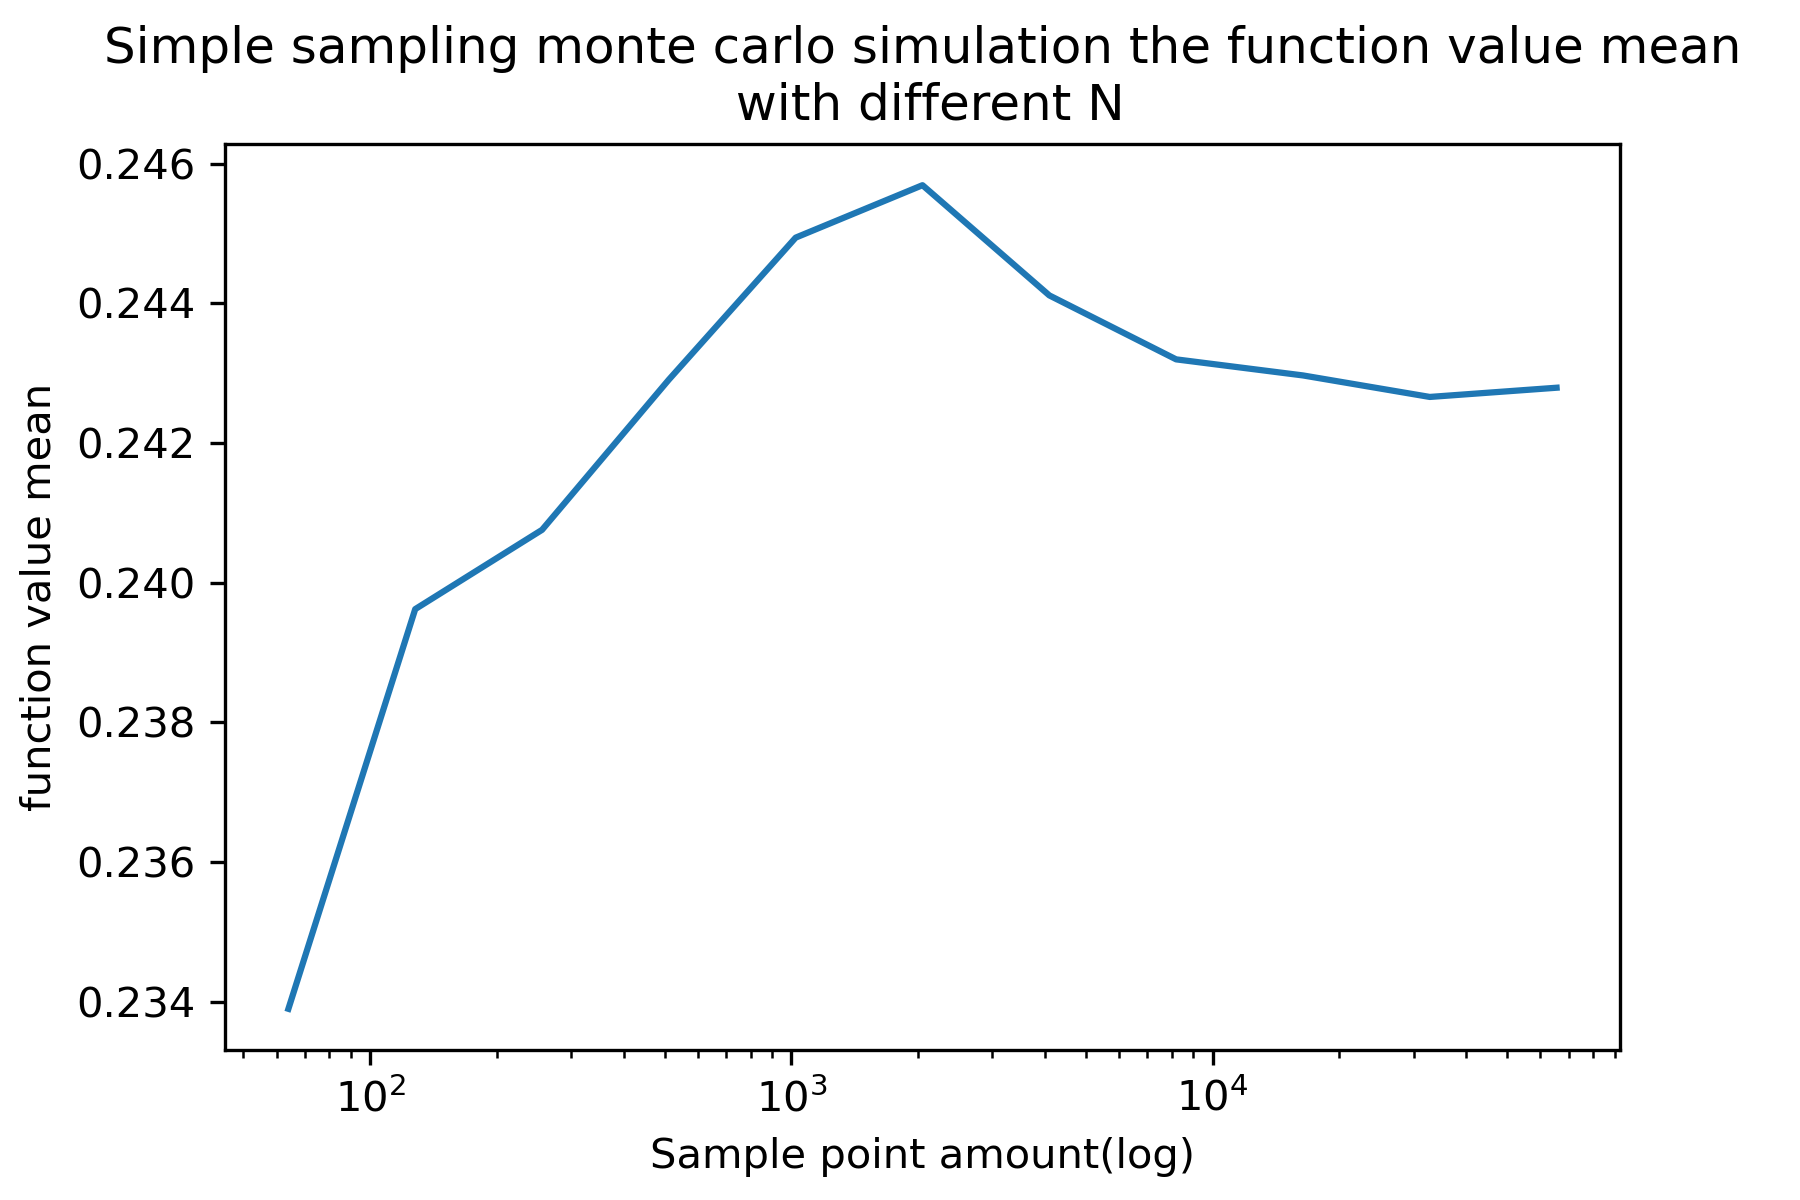
\includegraphics[width=0.9\linewidth]{notebook/ss_mean}
	\end{figure}
	\begin{figure}[hb!]
		\centering
		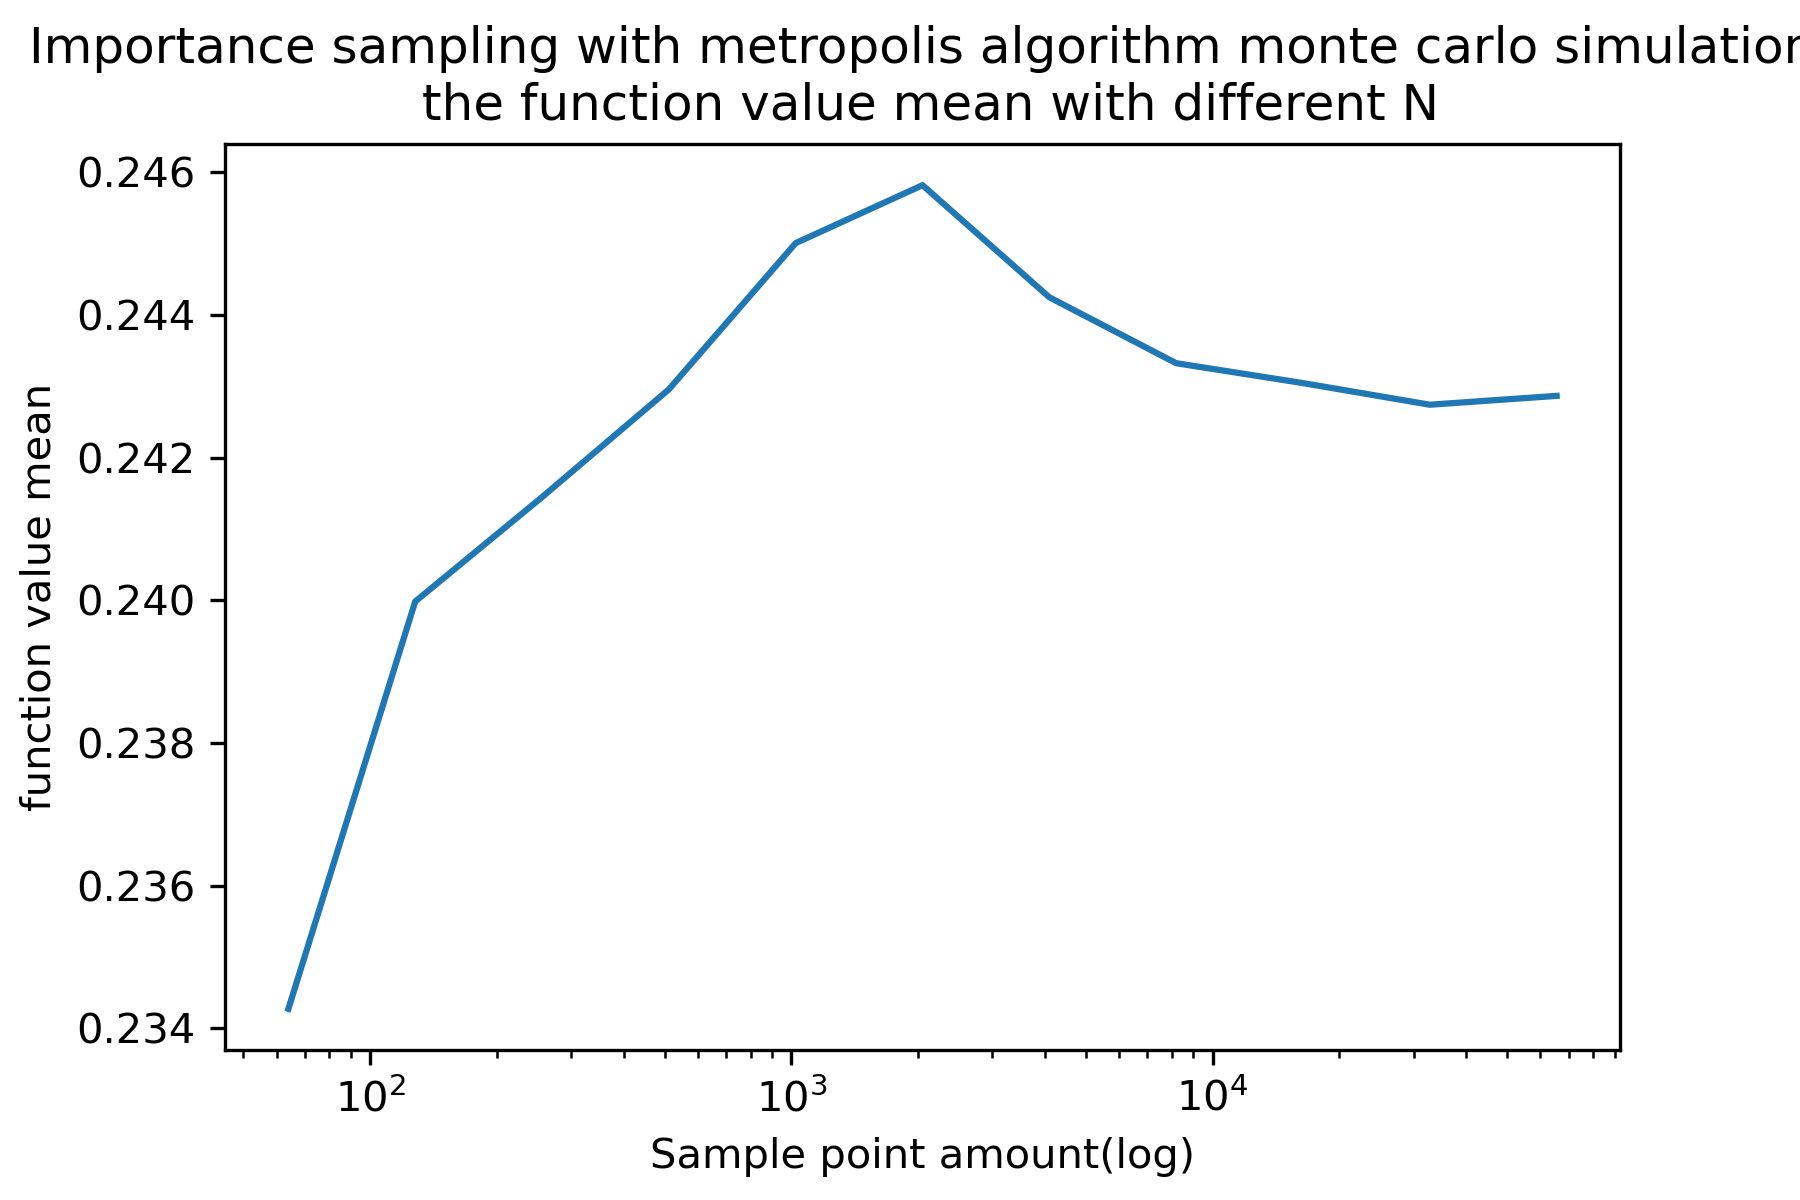
\includegraphics[width=0.9\linewidth]{notebook/mis_mean}
	\end{figure}

	The GPU calculation result (mean and standard deviation) of simple sampling monte carlo simulation is the same as CPU.


	The below two figure showed the function value standard deviation of both simple sampling monte carlo simulation and importance sampling with metropolis algorithm monte carlo simulation changing sample point amounts.
	\begin{figure}[hb!]
		\centering
		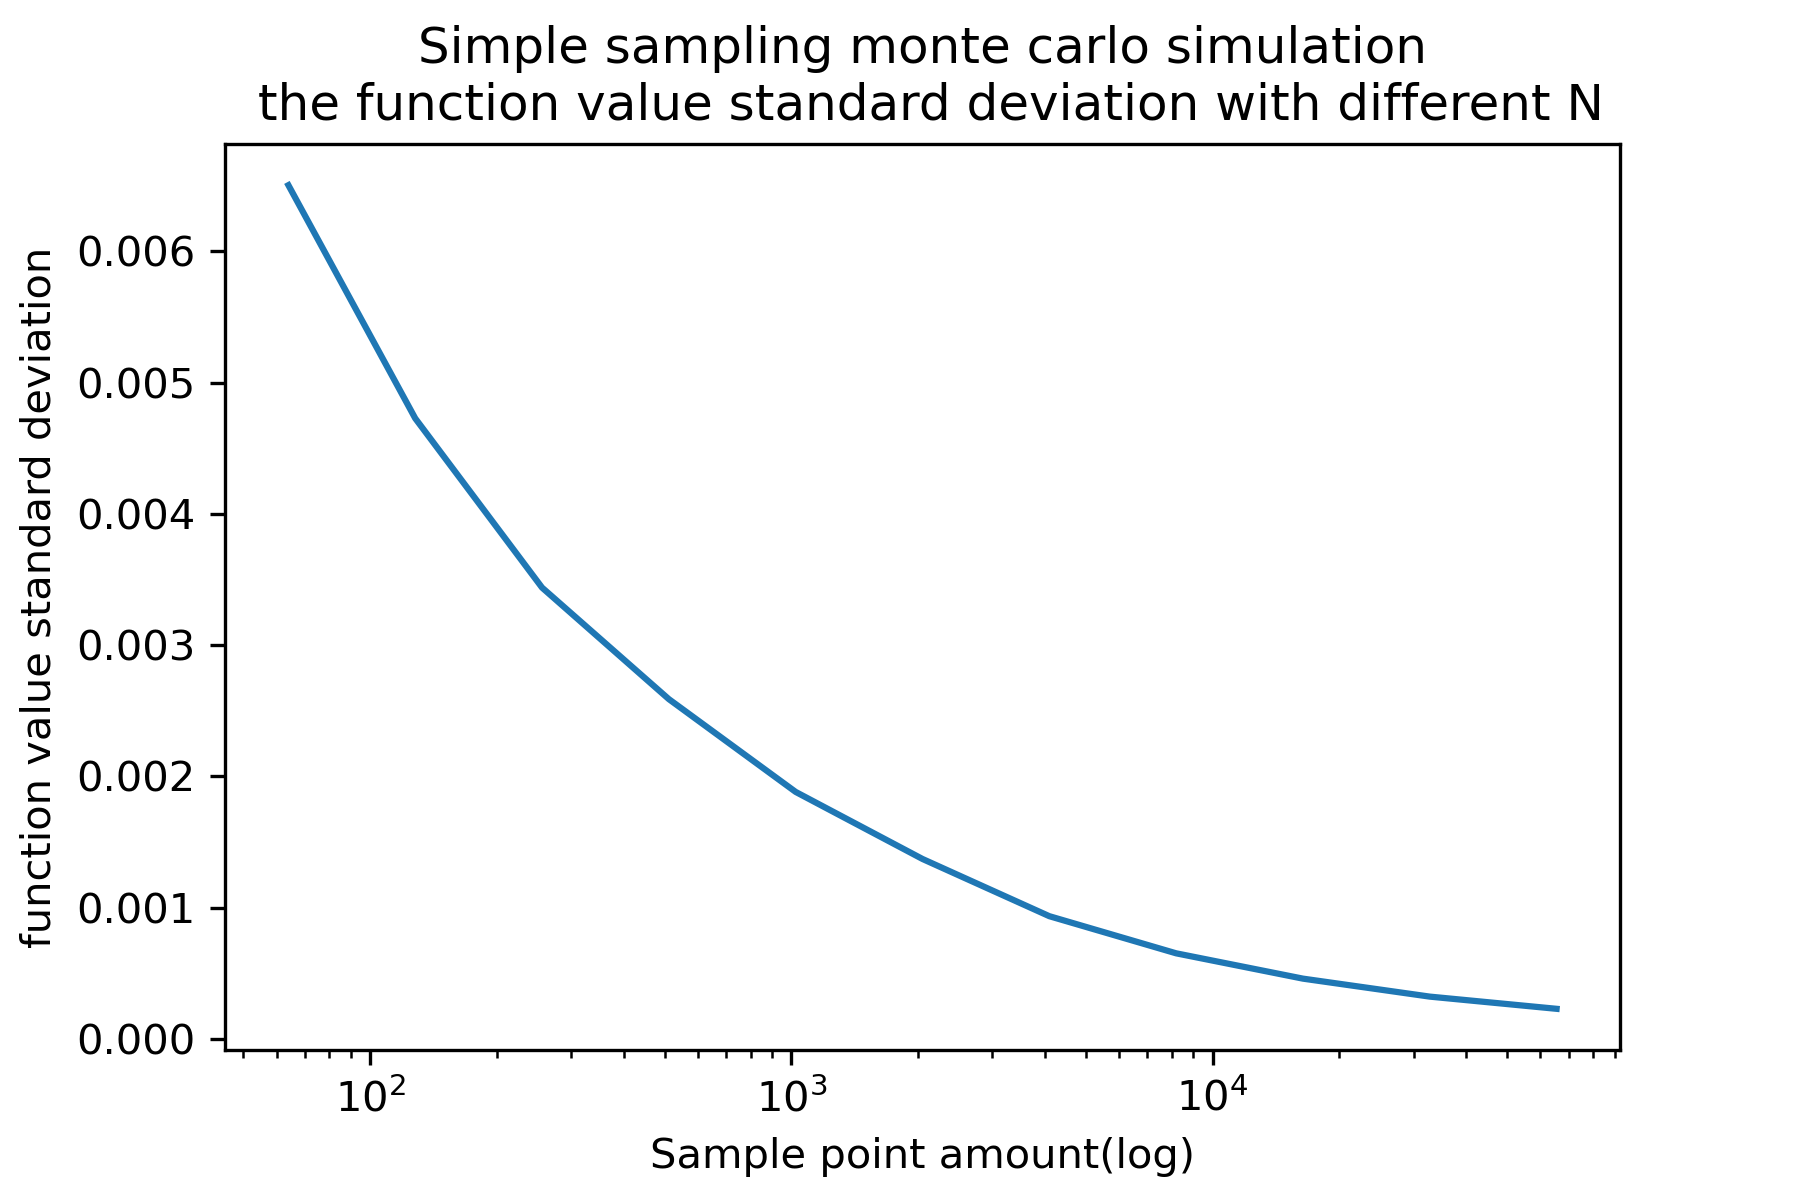
\includegraphics[width=\linewidth]{notebook/ss_std}
	\end{figure}
	\begin{figure}[hb!]
		\centering
		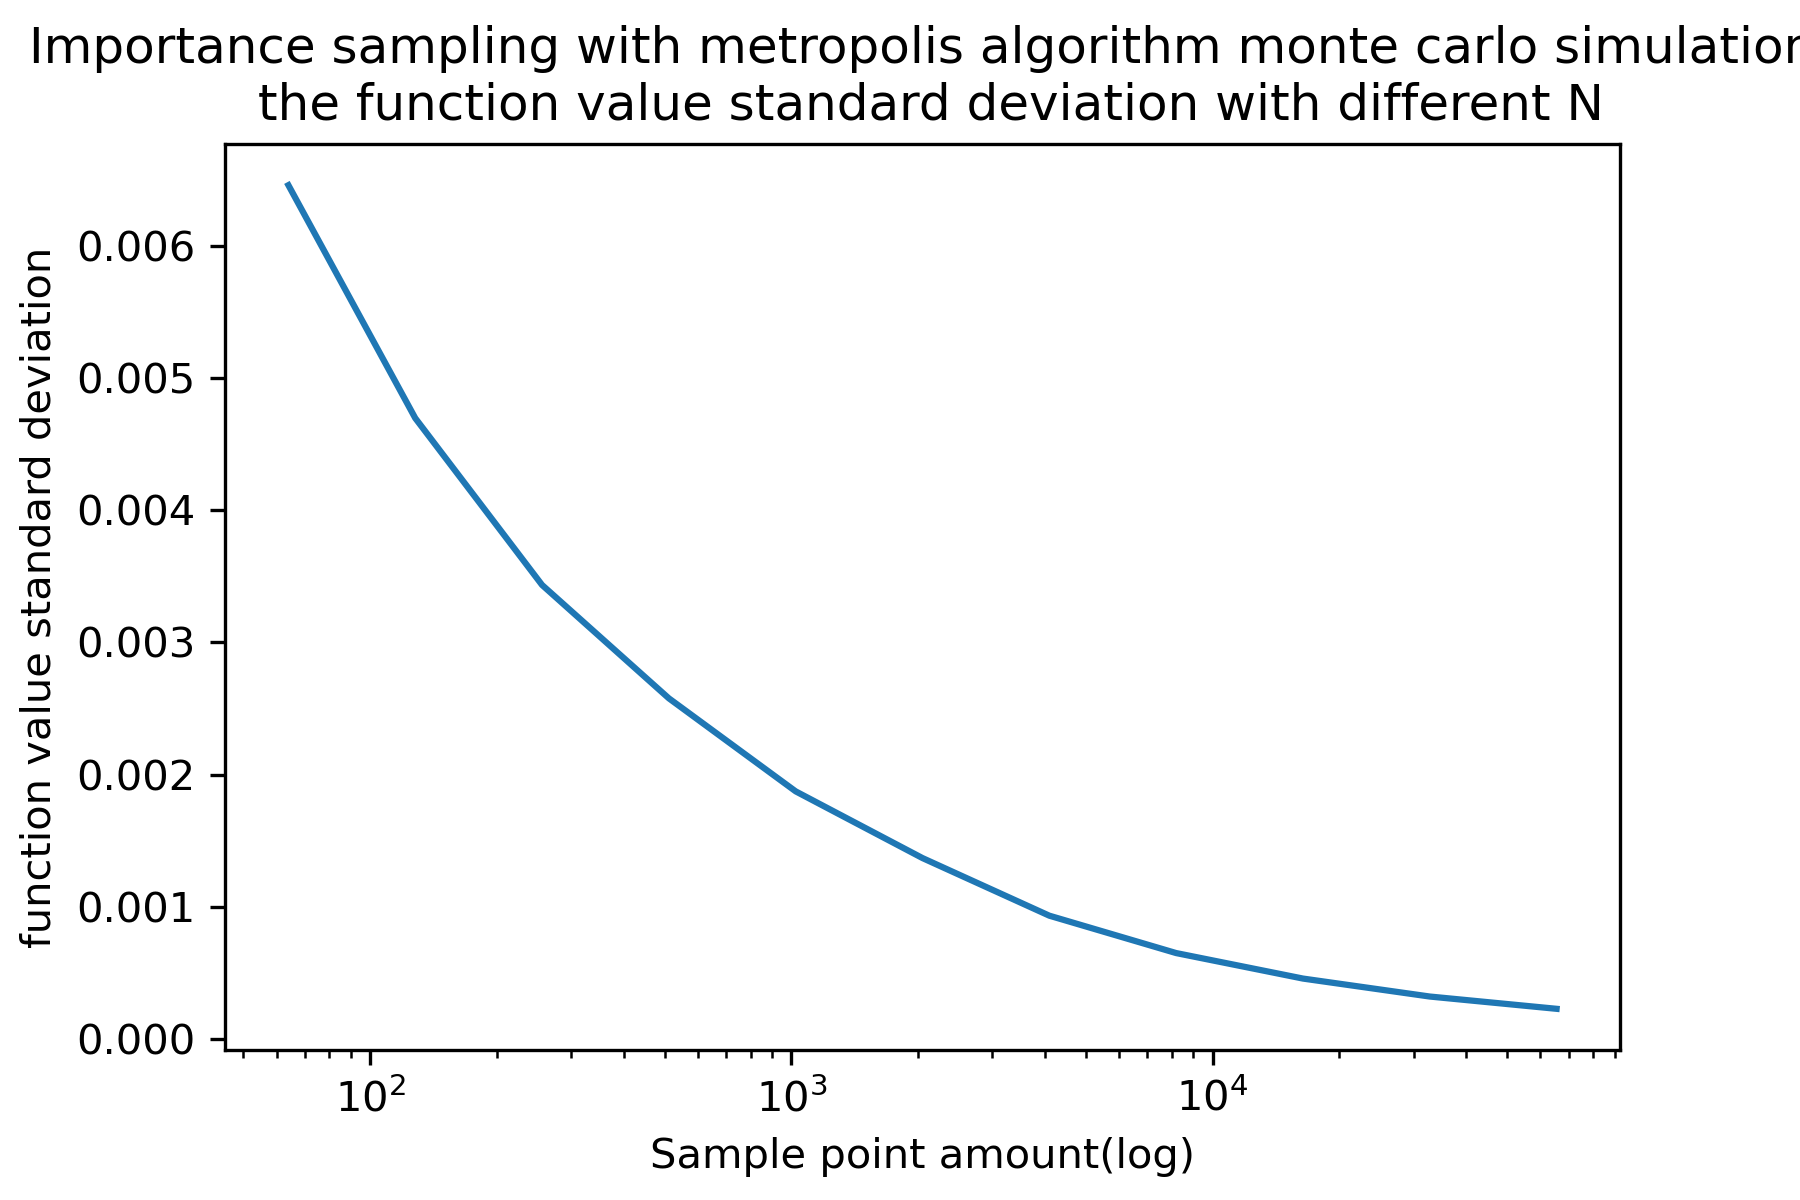
\includegraphics[width=\linewidth]{notebook/mis_std}
	\end{figure}


	And the below two figure showed the processing time of simple sampling monte carlo simulation and importance sampling with metropolis algorithm monte carlo simulation using 1 GPU and 2 GPU changing block size.
	\begin{figure}[hb!]
		\centering
		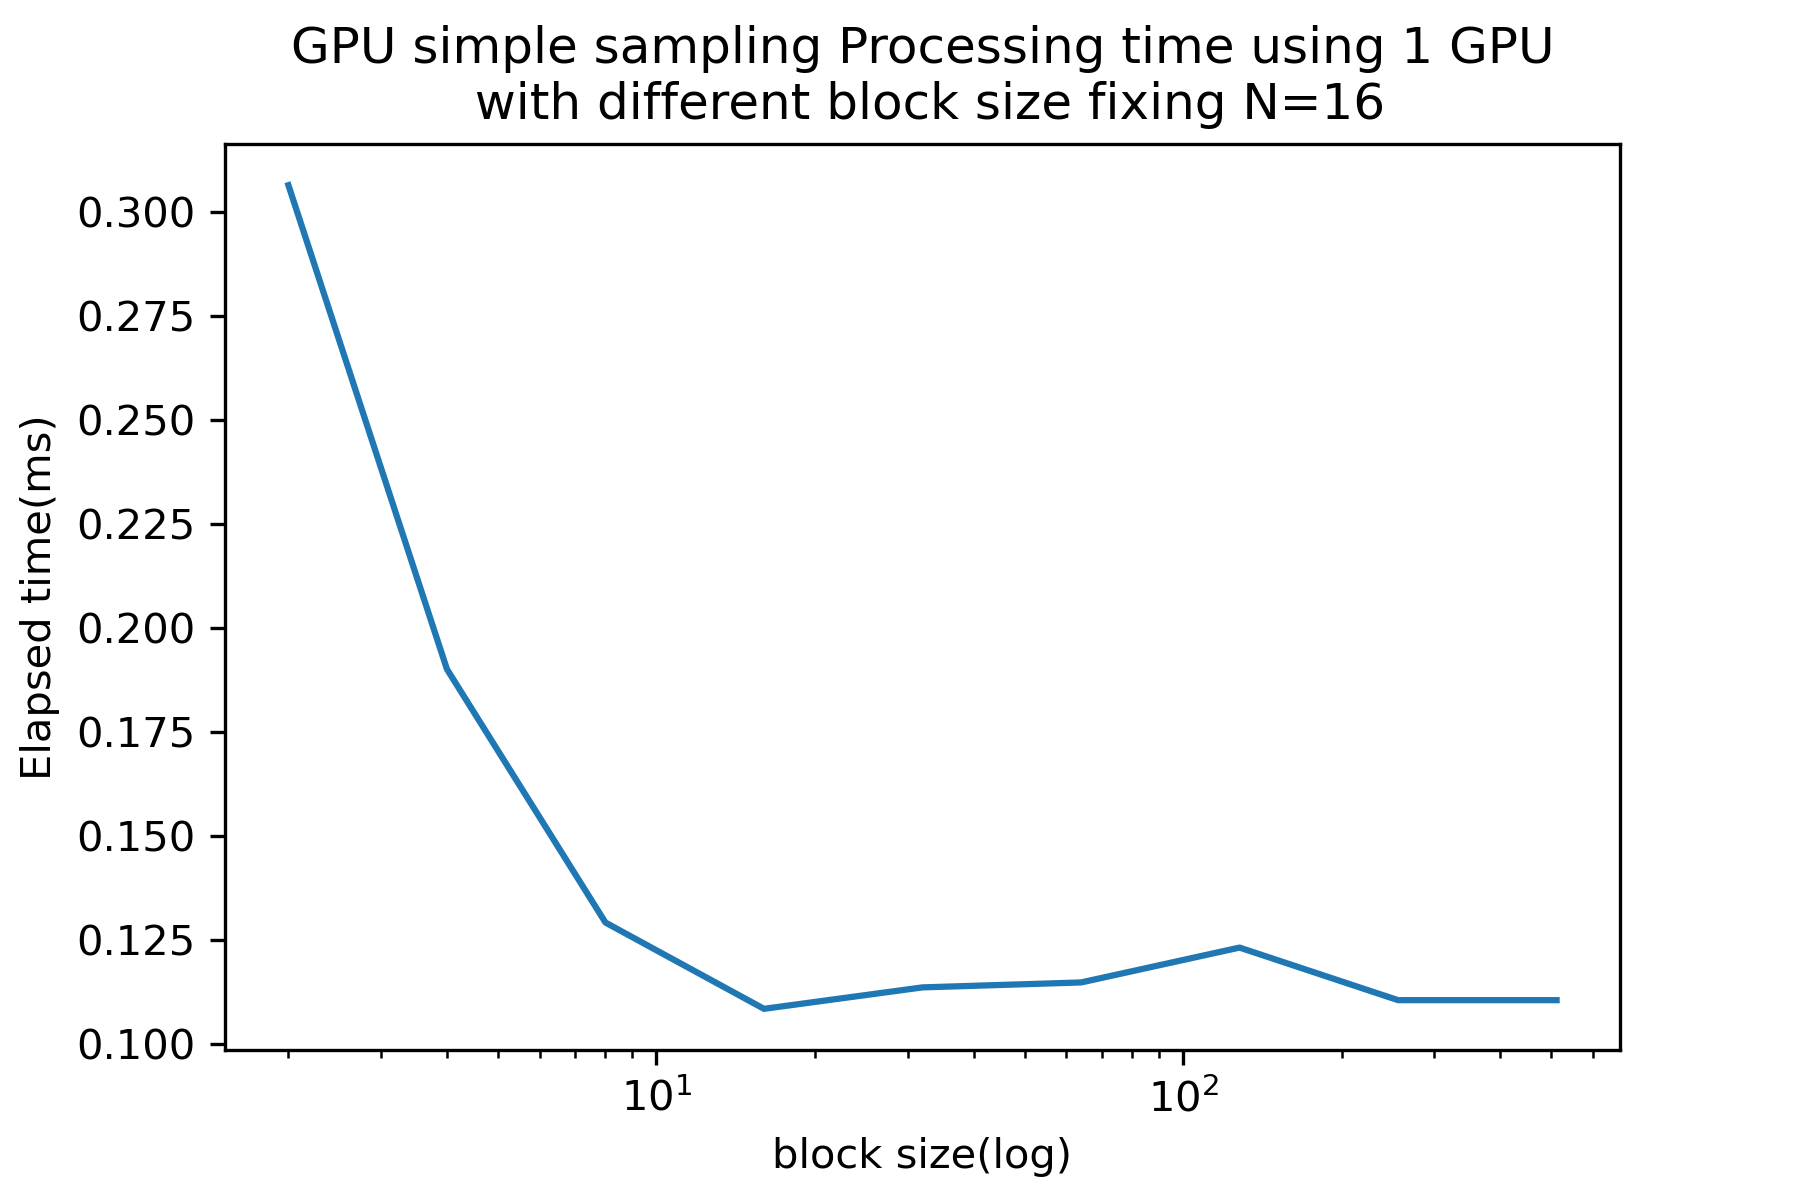
\includegraphics[width=\linewidth]{notebook/1gpu_ss_pt}
	\end{figure}
	\begin{figure}[hb!]
		\centering
		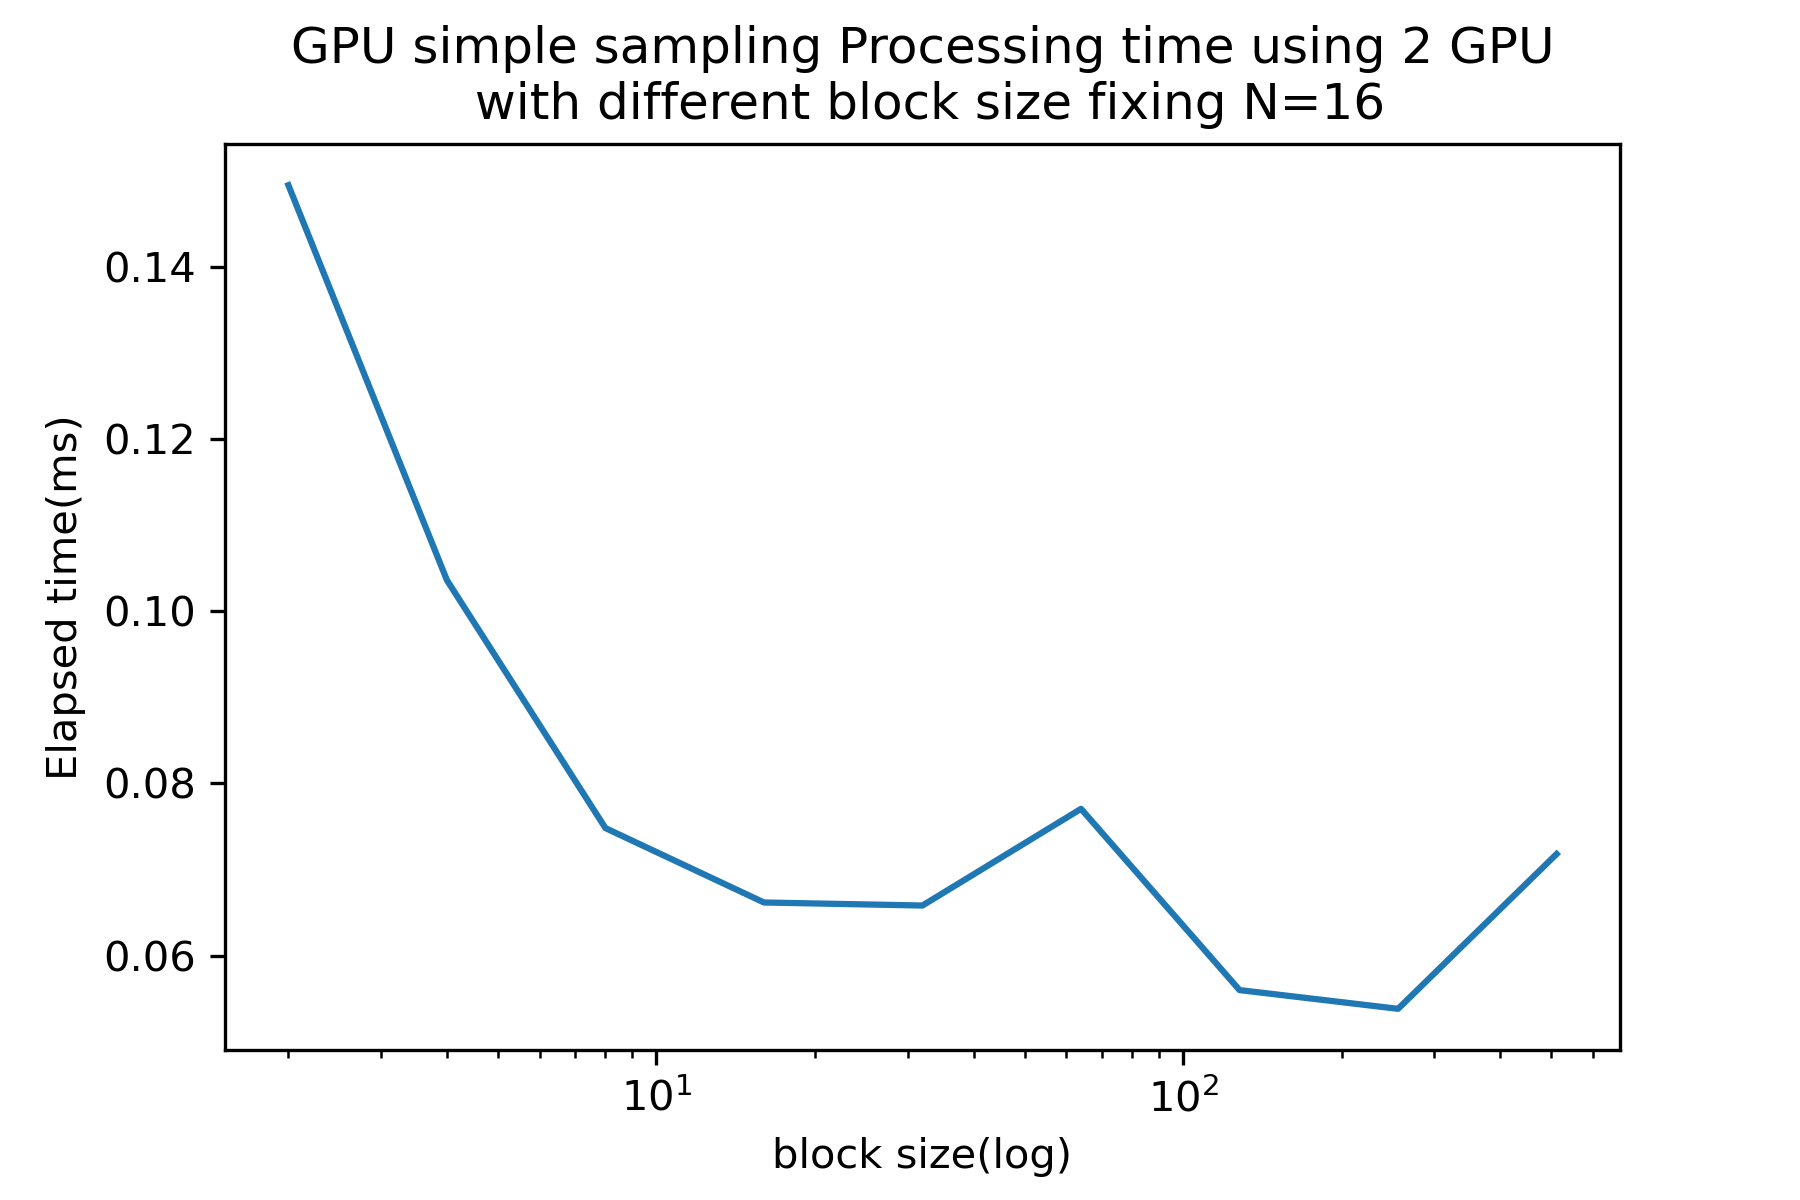
\includegraphics[width=\linewidth]{notebook/2gpu_ss_pt}
	\end{figure}

	\subsubsection{Observation}
	We can observe that the performance of small block size setup yield the worse performance in my experiment, and the computation performance increase until block size is large enough, its performance won't get any further increase after that. Through adding the sample point amount, the mean value becomes more stable and the standard variation becomes smaller, which roughly follows the inverse proportion to $\sqrt{N}$ where N is the sample points amount. 
	
	The importance sampling with metropolis algorithm monte carlo simulation have smaller standard deviation than the simple sampling one, this may due to the fact that it utilize the weighting function to smooth the original function.
		
	The optimal block size setup of calcutating the integral using simple sampling monte carlo simulation in my experiment are 8 block size for 1 GPU case, 8 block size(for small sample point case) and 256 block size(for large sample point case) for 2 GPU case.
	
	\section{Discussion}
	After experimenting a lot of times, I noticed that while performing importance sampling with metropolis algorithm monte carlo simulation, the weighting function should be designed carefully to make it normalize in the integral range, or the mean will be biased, which make the result weird.

\end{document}